\documentclass[a4paper, 12pt]{article}
\usepackage[total={17cm,25cm}, top=2.5cm, left=2.5cm, right=2.5cm,  includefoot]{geometry}
\usepackage[utf8]{inputenc}
\usepackage{array}
\usepackage{multirow}
\usepackage{hhline}
\usepackage{gensymb}
\usepackage{graphicx}
\graphicspath{ {} }
\usepackage[czech]{babel}
\usepackage{enumitem}
\usepackage{pdfpages}
\usepackage{amsmath}
\usepackage{verbatim}
\usepackage{listings}
\usepackage{hyperref}
\usepackage{amssymb}


\pagestyle{empty} % vypne číslování stránek




\usepackage[OT2,OT1]{fontenc}
\newcommand\cyr
{
\renewcommand\rmdefault{wncyr}
\renewcommand\sfdefault{wncyss}
\renewcommand\encodingdefault{OT2}
\normalfont
\selectfont
}
\DeclareTextFontCommand{\textcyr}{\cyr}
\def\cprime{\char"7E }
\def\cdprime{\char"7F }
\def\eoborotnoye{\char’013}
\def\Eoborotnoye{\char’003}


\begin{document}



\begin{titlepage}
\begin{center}
\noindent
\Large \textbf{České vysoké učení technocké v Praze}\\ Fakulta stavební
\vspace{5cm}

\huge

%vložení loga cvut
\begin{figure}[h!]
	\centering
	
\includegraphics[width=7cm]{logo.png}
\end{figure}

\vspace{0.5cm}

Algoritmy v digitální kartografii \\

\vspace{3cm}

\Huge  
Množinové operace s polygony\\

\vspace{2cm}

\Large
Bc. Robin Pflug \\
Bc. Tomáš Klemsa \\

\end{center}

\end{titlepage}




\pagestyle{plain}     % zapne obyčejné číslování
\setcounter{page}{1}  % nastaví čítač stránek znovu od jedné

\tableofcontents
\newpage

\section{Zadání úlohy}

\textbf{Vstup:} \textit{množina} $P=(P_1,...,P_n)$.\\
\textbf{Výstup:} 	\textit{množina polygonů $ P'=(P'_1,...,P'_m) $ } \\
\\
S využitím algoritmu pro množinové operace s polygony implementujte pro libovolné dva polygony $ P_i,P_j \epsilon P $ následující operace:

\begin{itemize}
\item Průnik polygonů $ P_i \cap P_j $,
\item Sjednocení polygonů $ P_i \cup P_j $,
\item Rozdíl polygonů $ P_i \cap \overline{P}_j $ resp $ P_j \cap \overline{P}_i $. .
\end{itemize}
Jako vstupní data použijte existující kartografická data (např. konvertované shape fily) či syntetické data, která budou načítána z textového souboru. \\
\\
Grafické rozhraní realizujte s využitím frameworku QT. \\
\\
Při zpracování se snažte postihnout nejčastější singulární případy: společný vrchol, společná část segmentu, společný celý segment čí více společných segmentů. Ošetřete situace, kdy výsledkem není 2D entita, ale 0D či 1D entita. \\
\\
Pro výše uvedené účely je nutné mít řádně odladěny algoritmy z úlohy 1. Postup ošetřená těchto případů diskutujte v technické zprávě, zamyslete se nad dalšími singularitami, které mohou nastat.

\begin{figure}[h!]
	\centering
	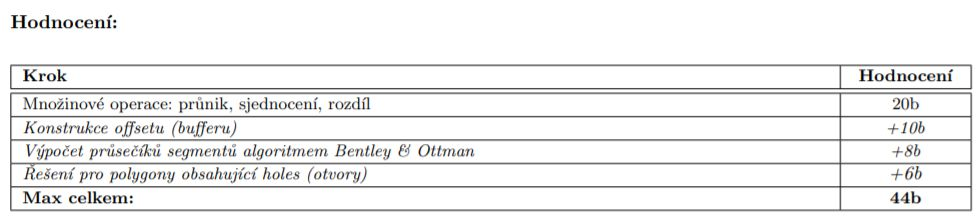
\includegraphics[width=12cm]{hodnoceni.jpg}
	\caption{Bodové ohodnocení úlohy [zdroj: 1]}
\end{figure}

\section{Údaje o bonusových úlohách}
Bonusové úlohy nebyly řešeny. Obsahem této úlohy je pouze povinná část zadání.

\newpage
\section{Obecná formulace a řešení problému}
Obsahem této úlohy je vytvořit aplikaci, která bude schopna provádět čtyři základní množinové operace nad dvěma zadanými polygony: průnik, sjednocení, a rozdíly.\\
\\
\textbf{Sjednocení množin:} $ A \cup B $\\ Sjednocením množin A a B vznikne nová množina, která bude obsahovat všechny prvky z množiny A a také všechny prvky z množiny B. [zdroj: 2]\\
\\
\textbf{Průnik množin:} $ A \cap B $\\ Průnikem dvou množin A a B vznikne nová množina, která bude obsahovat prvky, které mají ty dvě množiny společné. [zdroj: 2]\\
\\
\textbf{Rozdíl množin:} $ A \cap \overline{B} ; B \cap \overline{A} $\\ Rozdílem dvou množin A a B chápeme takovou množinu, která bude obsahovat všechny prvky z A a zároveň nebude obsahovat žádný prvek z B. Pro dva zadané polygony je tedy možné vyhodnotit jejich rozdíl dvěma způsoby \textit{(A-B nebo B-A)}. [zdroj: 2]

\begin{figure}[h!]
	\centering
	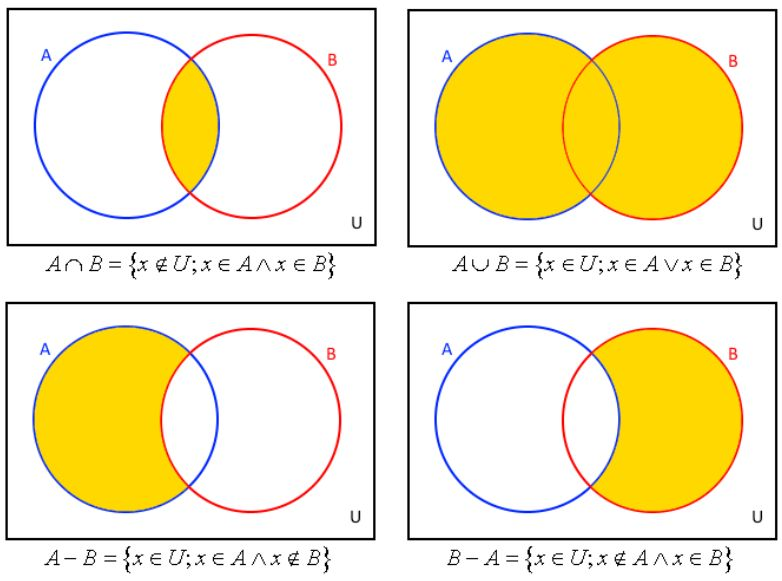
\includegraphics[width=12cm]{mnozinove_operace.jpg}
	\caption{Grafické znázornění jednotlivých množinových operací. [zdroj: 3]}
\end{figure}

\section{Aplikované algoritmy}
V aplikaci byly použity algoritmy pro vyhodnocení polohy bodu a přímky nebo polygonu, výpočet úhlu dvou vektorů, určení vztahu dvou přímek, výpočet průsečíků dvou polygonů. Aplikace algoritmů funguje pro nekonvexní polygony, kde výsledkem je prázdná množina, bod, přímka, plocha nebo kombinace těchto entit. 

\subsection{Výpočet průsečíků polygonů}
Pro výpočet průsečíků polygonu byl použit naivní algoritmus. Algoritmus postupně prochází všechny segmenty jednoho polygonu a porovnává je se všemi segmenty polygonu druhého. Pro případy, kdy existuje pro aktuální segment jednoho polygonu více průsečíků se segmenty polygonu druhého, není možné přidat mezi počáteční a koncový bod segmentu okamžitě nalezený průsečík. Je nutno nejprve nalézt všechny průsečíky náležící aktuálnímu segmentu a následně je přidávat ve správném pořadí. [zdroj 1]\\
\\
Pro tento krok je v aplikaci využita mapa. V mapě je jako klíč hodnota $\alpha$ nebo $\beta$ (\textit{poloha průsečíku na přímce}) a bod průsečíku. Pokud je nalezen nový bod, je seznam souřadnic bodů polygonu aktualizován na základě právě hodnoty klíče mapy. Tento postup zajistí zápis bodů ve správném pořadí. \\
\\
Poloha hrany vůči druhému polygonu je vyhodnocena na základě Winding number algoritmu a to tak, že je určována poloha středového bodu hrany vůči druhému polygonu. 

\begin{figure}[h!]
	\centering
	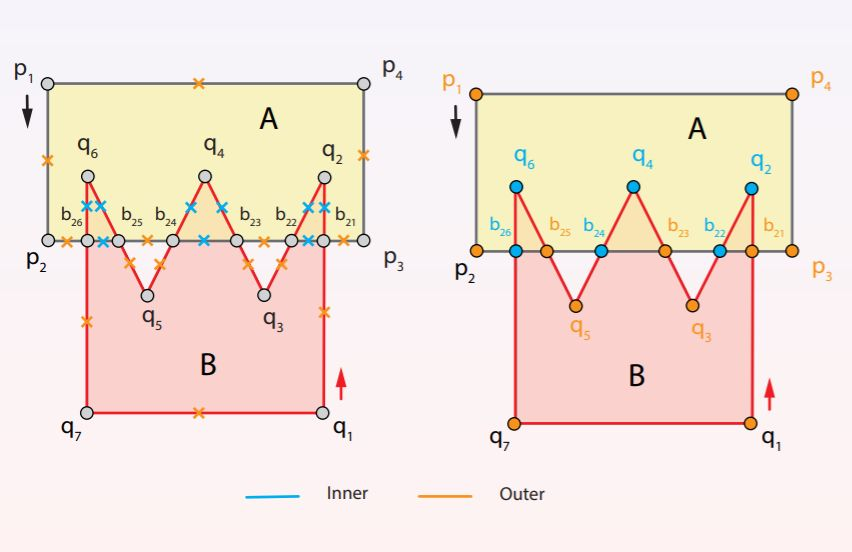
\includegraphics[width=12cm]{polygon_pruseciky.jpg}
	\caption{Příklad ohodnocení středů hran dvou polygonů. [zdroj: 1]}
\end{figure}

\subsubsection{Algoritmus Process intersection}
\begin{enumerate}
\item $ if (t >= \epsilon \land t <= 1- \epsilon): $ 
	\item \hspace {1cm} $ i \longleftarrow i+1 $
	\item \hspace {1cm}  $ P \longleftarrow (begin + i,pi)$ // Přidej průsečík na pozici i+1
\end{enumerate}[zdroj: 1]

\newpage
\subsubsection{Algoritmus pro výpočet průsečíků polygonů}
\begin{enumerate}
\item $ for (i = 0; i < n, i++) $ 
\item \hspace {1cm} $ intersections = map (double, QPointFB) $ // Vytvoření mapy 
\item \hspace {1cm} $ for (j = 0; j < m, j++) $
\item \hspace {2cm} if $ b_{ij} = (p_i, p_{(i+)1\%n} \cap q_j, q_{(j+)1\%m }) \neq 0$ // Existuje průsečík
\item \hspace {3cm} $ intersections [\alpha_i] \longleftarrow b_{ij}$ //Přidej do intersections
\item \hspace {3cm} processIntersection $ (b_{ij}, \beta, B, j) $ //Zpracuj první průsečík pro $ e_j $
\item \hspace {1cm} if $(||intersections|| > 0)$ // Nějaké průsečíky jsme nalezli
\item \hspace{2cm} $  for \forall m \in intersections: $ // Procházej všechny průsečíky v intersections
\item  \hspace{3cm} $ b \longleftarrow intersections.second $ // Získej 2. hodnotu z páru
\item \hspace{3cm} ProcessIntersection $ (b, \alpha, A, i) $ //Zpracuj první průsečík pro $ e_i $
\end{enumerate}

\subsubsection{Algoritmus pro polohu středového bodu hrany}
\begin{enumerate}
	\item for $(i = 0; i < n, i++)$:
	\item \hspace{1cm}$ M = \frac{p_i(x,y)+p_{i+1}(x,y)}{2}$ // Výpočet středu hrany
	\item \hspace{1cm}pozice = \textit{ positionPointPolygonWinding($\bar{p},B$)} //Určení polohy M.
	\item \hspace{1cm}$p_i[pozice]$ = pozice
\end{enumerate}

\subsection{Množinové operace}
Výsledný algoritmus množinových operací je založen na kombinaci algoritmů z předešlých kapitol.

\subsubsection{Algoritmus selecEdges}
\begin{enumerate}
	\item $for(\forall P[i])$
	\item \hspace{1cm} if$(P[i]_{position} = position)$ //Pokud je pozice bodu rovna hledané pozici
	\item \hspace{2cm} $e \leftarrow (P[i], P[i+1])$ //Vytvoř danou hranu
	\item $edges \leftarrow e$
\end{enumerate}

\subsubsection{Algoritmus boolean operations}

\begin{enumerate}
	\item computePolygonIntersection(PA, PB) //Nalezení průsečíků polygonů
	\item setPositionAB; //Nastavení hran
	\item if (Union)
	\item \hspace{1cm} seletEdges(PA, Outer)
	\item \hspace{1cm} selectEdges(PB, Outer) //Sjednocení
	\item if (Intersect)
	\item \hspace{1cm} seletEdges(PA, Inner)
	\item \hspace{1cm} selectEdges(PB, Inner) //Průnik
	\item if (DiffAB)
	\item \hspace{1cm} seletEdges(PA, Outer)
	\item \hspace{1cm} selectEdges(PB, Inner) //Rozdíl AB
		\item if (Union)
	\item \hspace{1cm} seletEdges(PA, Inner)
	\item \hspace{1cm} selectEdges(PB, Outer) //Rozdíl BA	
\end{enumerate}

\subsubsection{Algoritmus setPositionAB}
\begin{enumerate}
\item poloha bodů středů hran pro PA,PB
\item poloha bodů středů hran pro PB,PA
\end{enumerate}

\newpage

\section{Problémové vstupní množiny}
Vstupní množiny vytvářející polygony mohou obsahovat singulární případy. Testované singulární případy jsou situace, kdy mají polygony společný jeden nebo více vrcholů a jednu nebo více hran.\\
\\
Pro první možnost (společný jeden bod), kdy je požadavek Intersect, vrátí aplikace prázdnou množinu hran. Ostatní množinové operace fungují ze své podstaty klasicky.

\begin{figure}[h!]
	\centering
	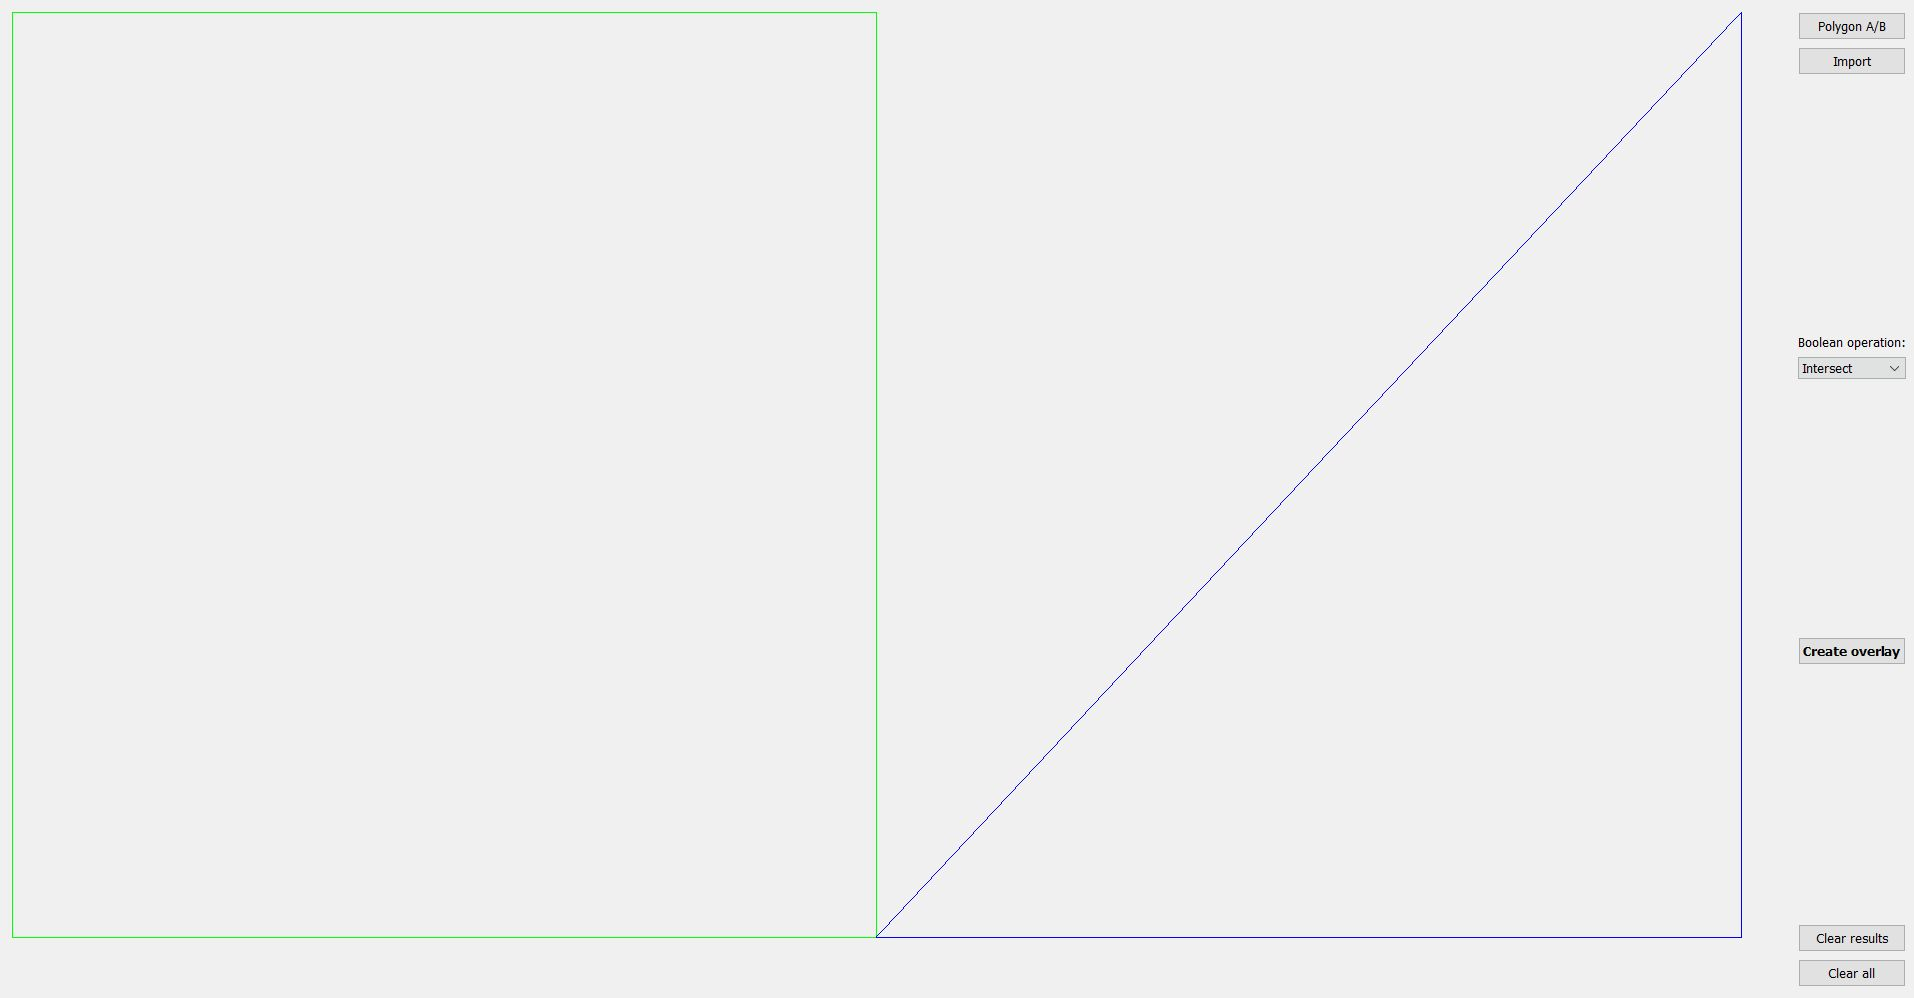
\includegraphics[width=12cm]{one_point.jpg}
	\caption{Příklad výstupu aplikace pro průnik množin se společným vrcholem}
\end{figure}

Pro případy, kdy je na vstupu množina bodů vytvářející polygony s jednou či více společnými hranami je opět zajímavý požadavek průniku množin. Aplikace navrací seznam hran obsahující právě tyto společné hrany.

\begin{figure}[h!]
	\centering
	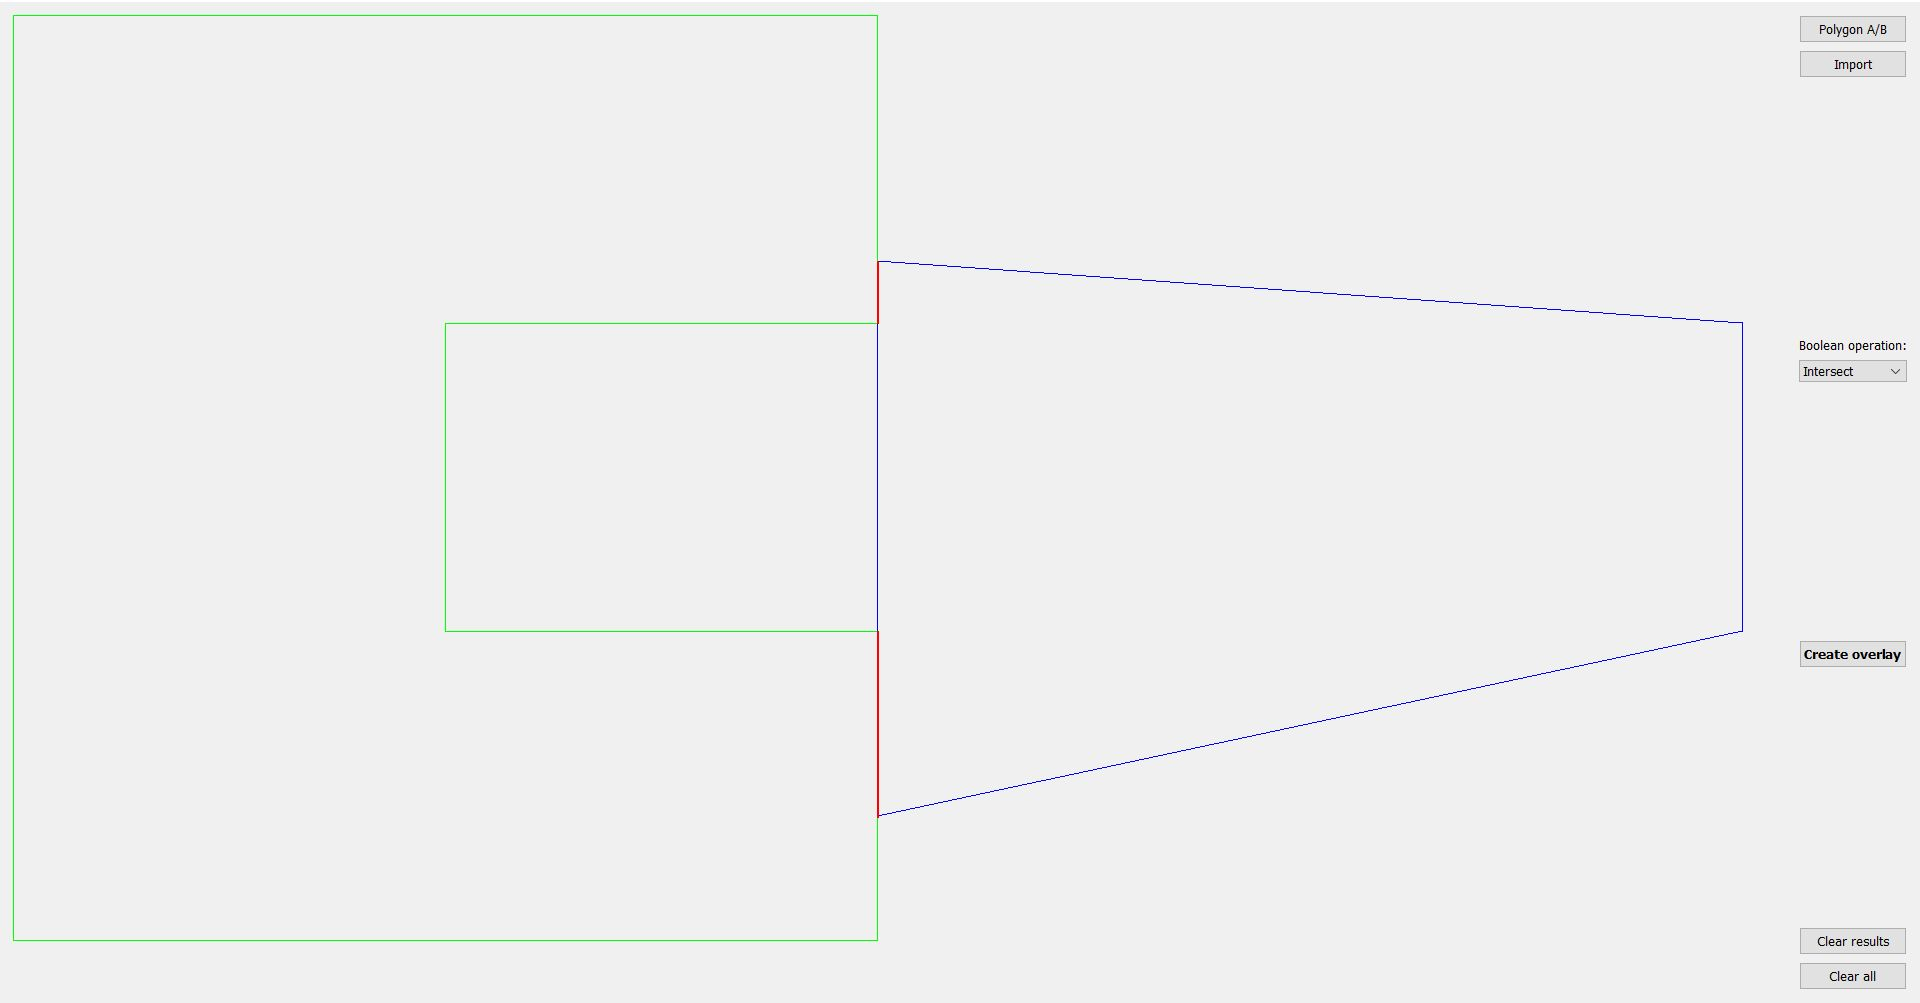
\includegraphics[width=12cm]{same_edges.jpg}
	\caption{Příklad výstupu aplikace pro průnik množin se společnými hranami}
\end{figure}

\newpage

\section{Vstup dat do aplikace}
Vstup dat do aplikace lze realizovat dvěma způsoby. Uživatel může graficky vkládat jednotlivé vrcholy polygonů přímo kurzorem myši (se zřetelem na topologickou korektnost). Změna příslušnosti budoucího vrcholu k polygonu lze měnit tlačítkem "Polygon $A/B$".\\
\\
Druhá možnost vstupu dat do aplikace je formou importu souřadnic vrcholů polygonu. Importovaný soubor ve formátu txt musí být ve formátu: \textit{čísloPolygonu souřadniceX souřadniceY} . Pořadí vrcholů polygonu určuje také pořadí vytvořených hran.\\
\\
 
\begin{figure}[h!]
	\centering
	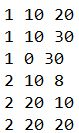
\includegraphics[width=1.5cm]{data.jpg}
	\caption{Vzor vstupních dat pro nahrávaní ze souboru .txt}
\end{figure}

\section{Výstup aplikace}
Grafický výstup je prezentován v Canvasu grafického rozhraní.

\begin{figure}[h!]
	\centering
	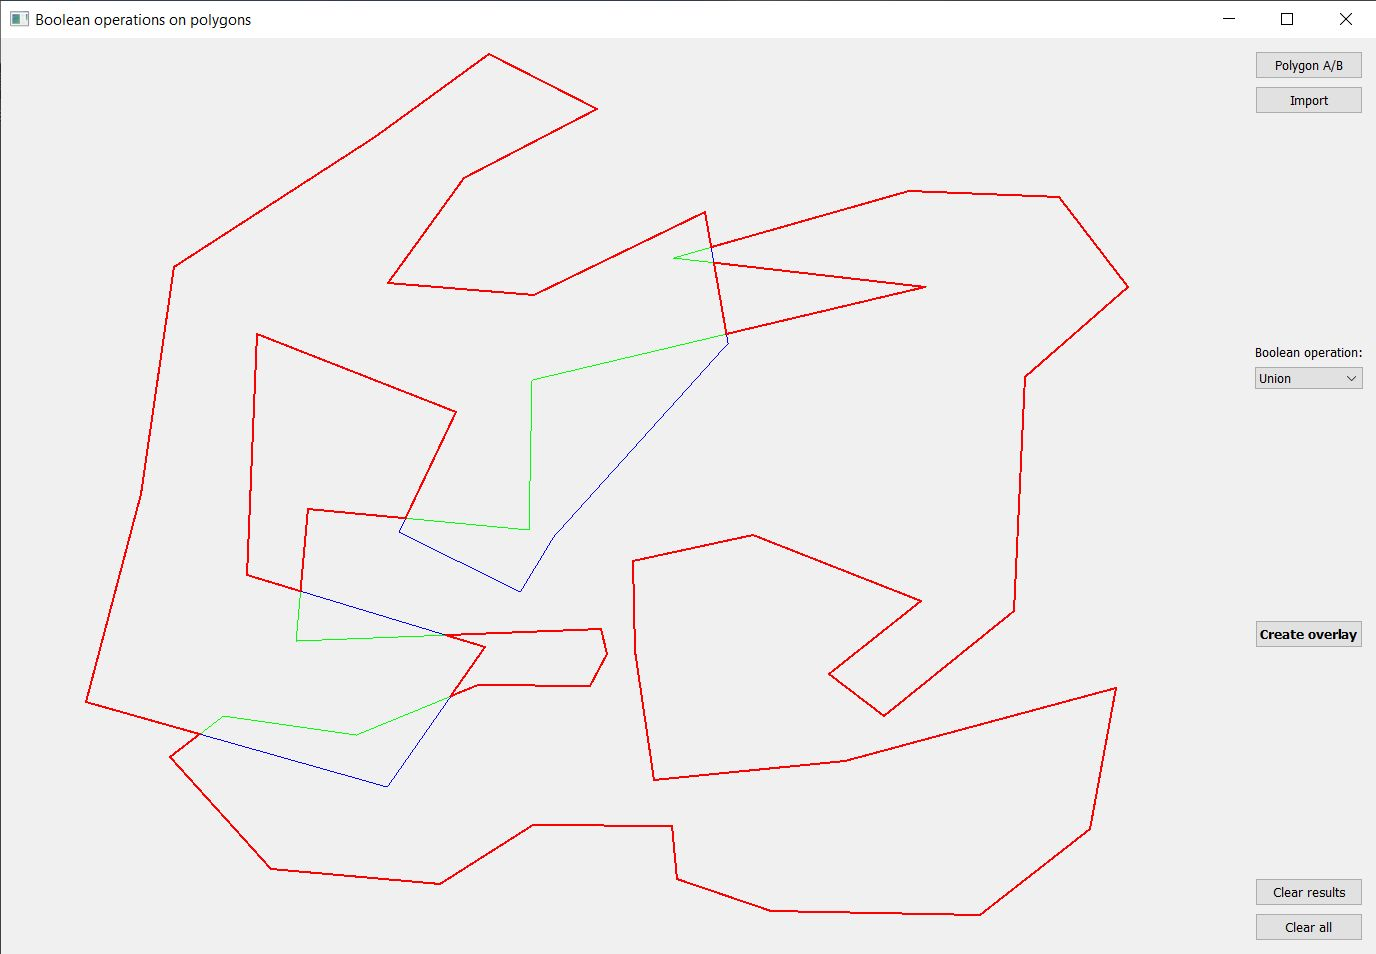
\includegraphics[width=12cm]{vystup.jpg}
	\caption{Příáklad výstupu aplikace pro zadané polygony s vyhodnocením jejich sjednocení}
\end{figure}

\section{Dokumentace}
\subsection{Třídy}
\subsubsection{Algorithms}
Třída Algorithms obsahuje metody zajišťující výpočty daných algoritmů.\\
\\
\textbf{TPointLinePosition getPointLinePosition(QPointFB q, QPointFB p1, QPointFB p2)}\\
Návratová hodnota: \textit{TPointLinePosition};\\
Metoda vyhodnocující polohu bodu vůči zadané přímce. Metoda navrací hodnoty \textit{LeftHp}(bod v lévé polorovině), \textit{RightHp}(bod v pravé polorovině),nebo \textit{Colinear}(bod na přímce). \\
\\
\textbf{double getAngle2Vectors(QPointFB p1, QPointFB p2, QPointFB p3, QPointFB p4)}\\
Návratová hodnota: \textit{double};\\
Metoda navrací hodnotu úhlu mezi dvěma vektory.\\
\\
\textbf{TPointPolygonPosition positionPointPolygonWinding(QPointFB q, std::vector$<QPointFB>$ pol)}\\
Návratová hodnota: \textit{TPointPolygonPosition};\\
Metoda určující vzájemnou polohu bodu a polygonu algoritmem Winding number.Metoda navrací hodnoty \textit{Inner}(bod uvnitř), \textit{Outer}(bod vně),nebo \textit{On}(bod na hraně). \\
\\
\textbf{T2LinesPosition get2LinesPosition(QPointFB p1, QPointFB p2, QPointFB p3, QPointFB p4, QPointFB pi)}\\
Návratová hodnota: \textit{T2LinesPosition};\\
Metoda vyhodnocující vzájemný vztah dvou přímek. Metoda navrací hodnoty \textit{Paralel}(rovnoběžné přímky), \textit{Identical}(přímky se překrývají), \textit{NonIntersected}(přímky nemají společný bod), nebo \textit{Intersected}(přímky mají společný bod). \\
\\
\textbf{vector$<Edge>$ booleanOperations(vector$<QPointFB>$ polygonA,vector$<QPointFB>$ polygonB, TBooleanOperation operation)}\\
Návratová hodnota: \textit{vector$<Edge>$};\\
Metoda vrátí vektor hran, které jsou výsledkem zadané boolean operace.\\ 
\\
\textbf{void processIntersection(QPointFB pi, double t, std::vector<QPointFB> polygon, int i)}\\
Návratová hodnota: \textit{void};\\
Metoda přidá bod do listu vrcholů polygonů, pokud zatím neexistuje.\\
\\
\textbf{void computePolygonIntersection(vector$<QPointFB>$ pa, vector$<QPointFB>$ pb)}\\
Návratová hodnota: \textit{void};\\
Metoda vypočte průsečíky hran polygonů.\\
\\
\\
\textbf{void setPositionsAB(vector$<QPointFB>$ pa, vector$<QPointFB>$ pb)};\\
Návratová hodnota: \textit{void};\\
Metoda nastaví vztah hran vůči druhému polygonu u obou polygonů.\\
\\
\textbf{void setPositions(vector$<QPointFB>$ pa, vector$<QPointFB>$ pb)};\\
Návratová hodnota: \textit{void};\\
Metoda provádí výpočet vztahu hran polygonu vůči druhému.\\
\\
\textbf{void selectEdges(vector$<QPointFB>$ pol, TPointPolygonPosition position, vector$<Edge>$ edges)}\\
Návratová hodnota: \textit{void};\\
Metoda naplní vektor hran na základě požadavku na jejich pozici. 

\subsubsection{Edge}
Třída Edge definuje hranu. Hrana je dána jako počáteční bod \textit{s} a koncový bod \textit{e}.\\
\\
\textbf{QPointFB getStart()}\\
Návratová hodnota: \textit{QPointFB};\\
Metoda vracející počáteční bod linie.\\
\\
\textbf{QPointFB getEnd()}\\
Návratová hodnota: \textit{QPointFB};\\
Metoda vracející koncový bod linie.\\
\\
\textbf{void setStart(QPointFB s)}\\
Návratová hodnota: \textit{void};\\
Metoda nastaví počáteční bod linie.\\
\\
\textbf{void setEnd(QPointFB e)}\\
Návratová hodnota: \textit{void};\\
Metoda nastaví koncový bod linie.

\subsubsection{QPointFB}
Třída QPointFB definuje bod o souřadnicích x a y. Dalé body uchovávají hodnotu alfa a beta (jejich pozice na přímce polygonů) a také hodnotu polohy vůči přímce (x; y; alpha; beta; position).\\
\\
\textbf{double getAlpha()}\\
Návratová hodnota: \textit{double};\\
Metoda vracející hodnotu alfa.\\
\\
\textbf{double getBeta()}\\
Návratová hodnota: \textit{double};\\
Metoda vracející hodnotu beta.\\
\\
\textbf{TPointPolygonPosition getPosition()}\\
Návratová hodnota: \textit{TPointPolygonPosition};\\
Metoda vracející polohu bodu vůči přímce.\\
\\
\textbf{void setAlpha(double alpha)}\\
Návratová hodnota: \textit{void};\\
Metoda nastaví pro bod \textit{QPointFB} hodnotu \textit{alfa}.\\
\\
\textbf{void setBeta(double beta)}\\
Návratová hodnota: \textit{void};\\
Metoda nastaví pro bod \textit{QPointFB} hodnotu \textit{beta}.\\
\\
\textbf{void setPosition(TPointPolygonPosition position)}\\
Návratová hodnota: \textit{void};\\
Metoda nastaví pro bod \textit{QPointFB} polohu vůči přímce.

\section{Testování}
Testování probíhalo na syntetických datech vytvořených v textovém editoru. Další způsob zadávání množin bodů pro testování bylo realizováno přímo grafickým vstupem.

\subsection{Test 1}
První testování bylo provedeno na množině obsahující řádově desítky vrcholů polygonů. Množina byla vytvořena grafickým vstupem. Pro všechny množinové operace dávala aplikace správné výsledky.
 \begin{figure}[h!]
	\centering
	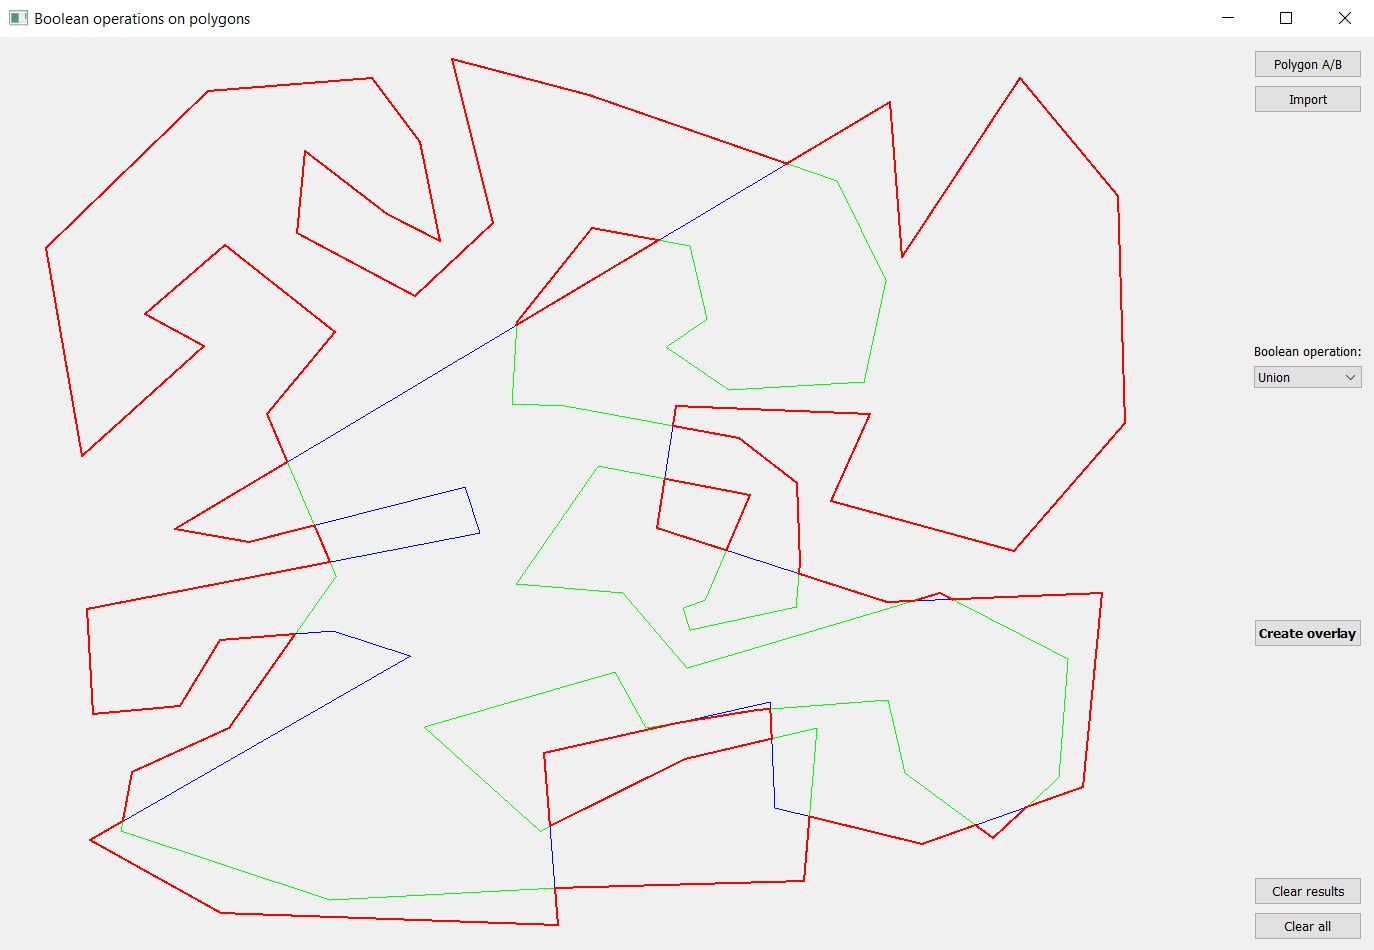
\includegraphics[width=9cm]{t1.jpg}
	\caption{Union}
\end{figure}

 \begin{figure}[h!]
	\centering
	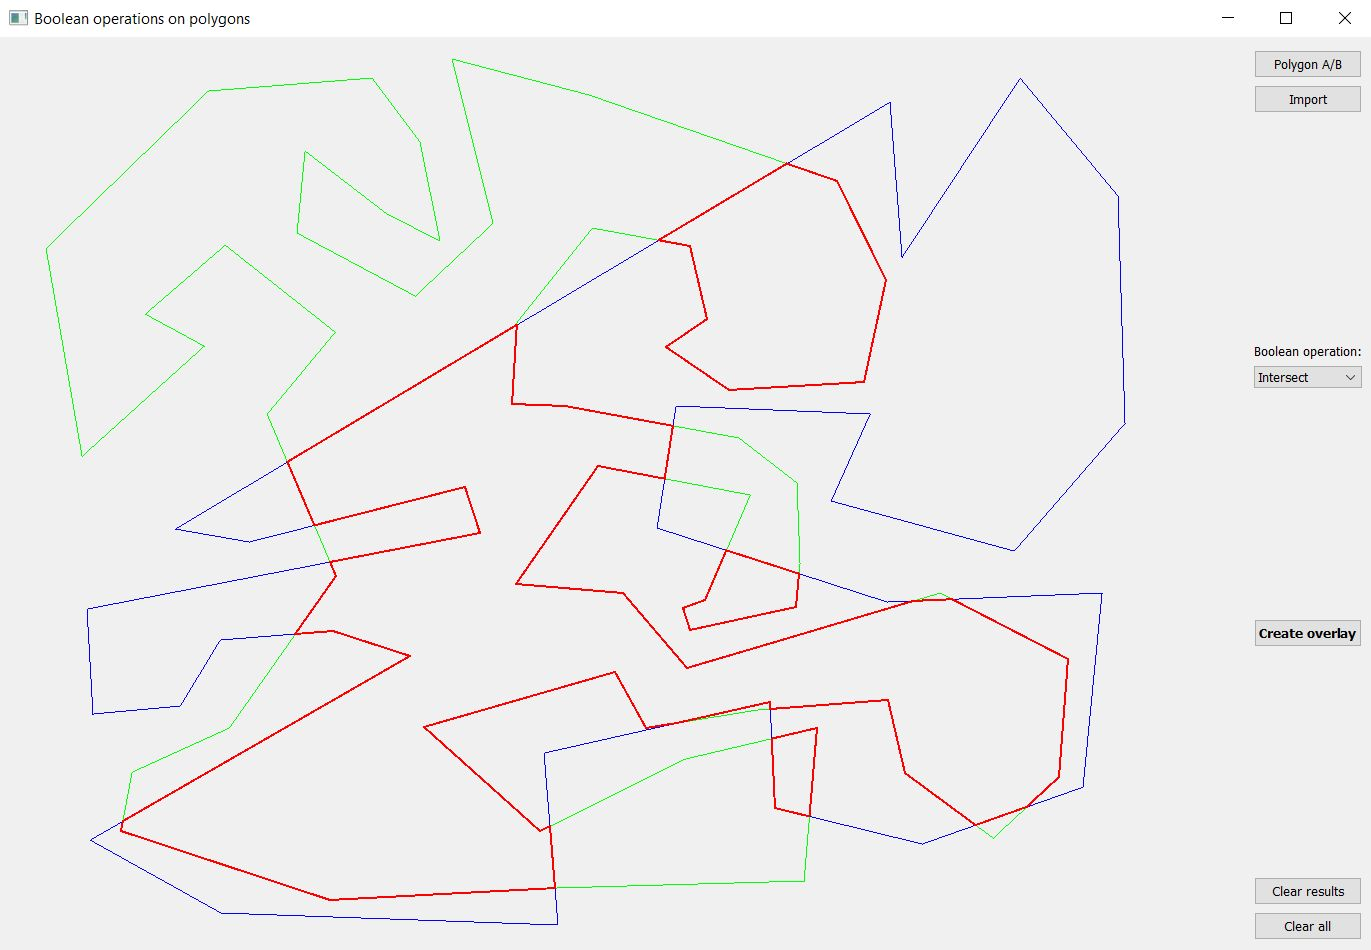
\includegraphics[width=9cm]{t2.jpg}
	\caption{Intersect}
\end{figure}

 \begin{figure}[h!]
	\centering
	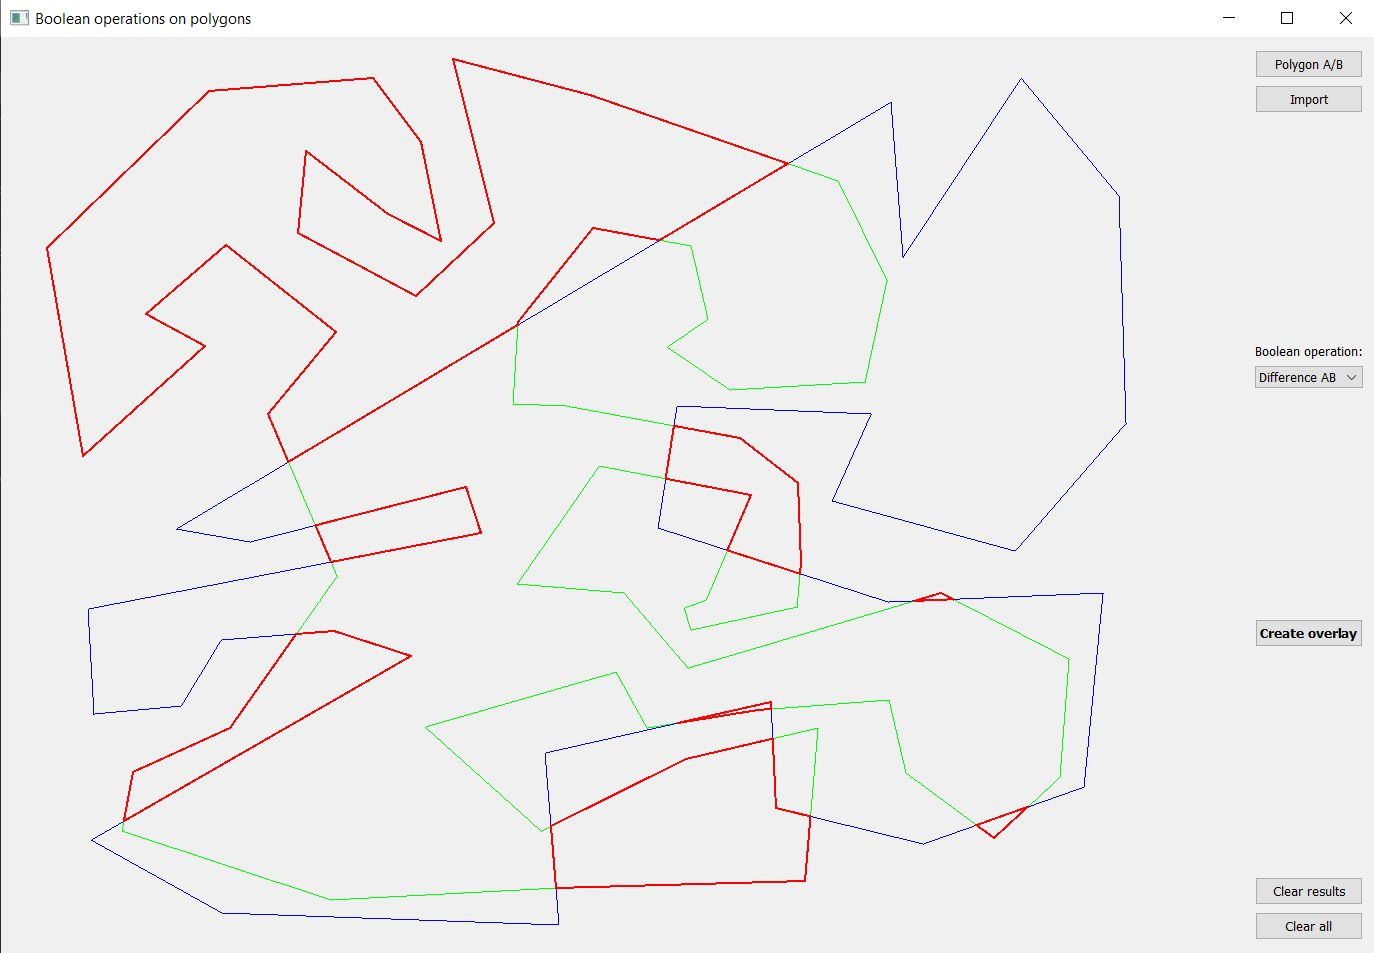
\includegraphics[width=9cm]{t3.jpg}
	\caption{Difference AB}
\end{figure}

 \begin{figure}[h!]
	\centering
	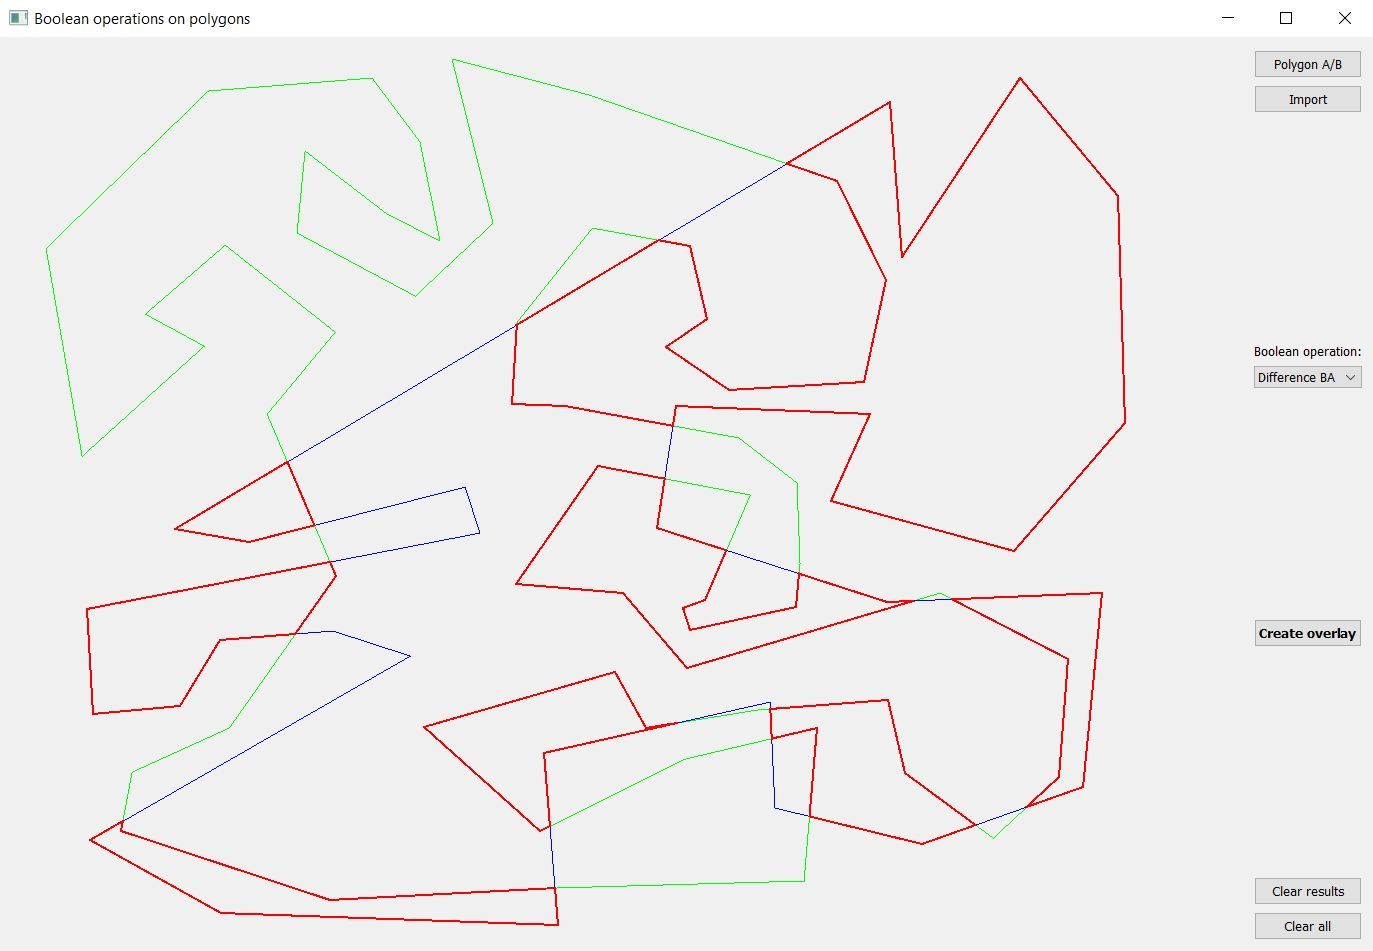
\includegraphics[width=9cm]{t4.jpg}
	\caption{DifferenceBA}
\end{figure}

\clearpage

\subsection{Test2}
Druhá množina použita pro testování dat byla vytvořena syntetiky v textovém editoru. Množina obsahovala dva polygony se dvěma společnými hranami. Aplikace dávala ve všech případech opět korektní řešení. Příklad výstupu tohoto testu je obsahem kapitoly \textit{5 Problémové vstupní množiny} 

\subsection{Test3}
Třetí množina použita pro testování dat obsahovala opět dva polygony. Jeden polygon ovšem obsahoval "díru". Pro tento polygon nebyla aplikace schopna správně vyhodnotit množinové operace. Možné úskalí je ve formátu, jakým je polygon načítán. Pro polygony nelze v aplikaci definovat prázdnou vnitřní oblast zvlášť. Proto aplikace vytvoří nekorektní linii, spojující obvod polygonu s vnitřní oblastí ("díra").

 \begin{figure}[h!]
	\centering
	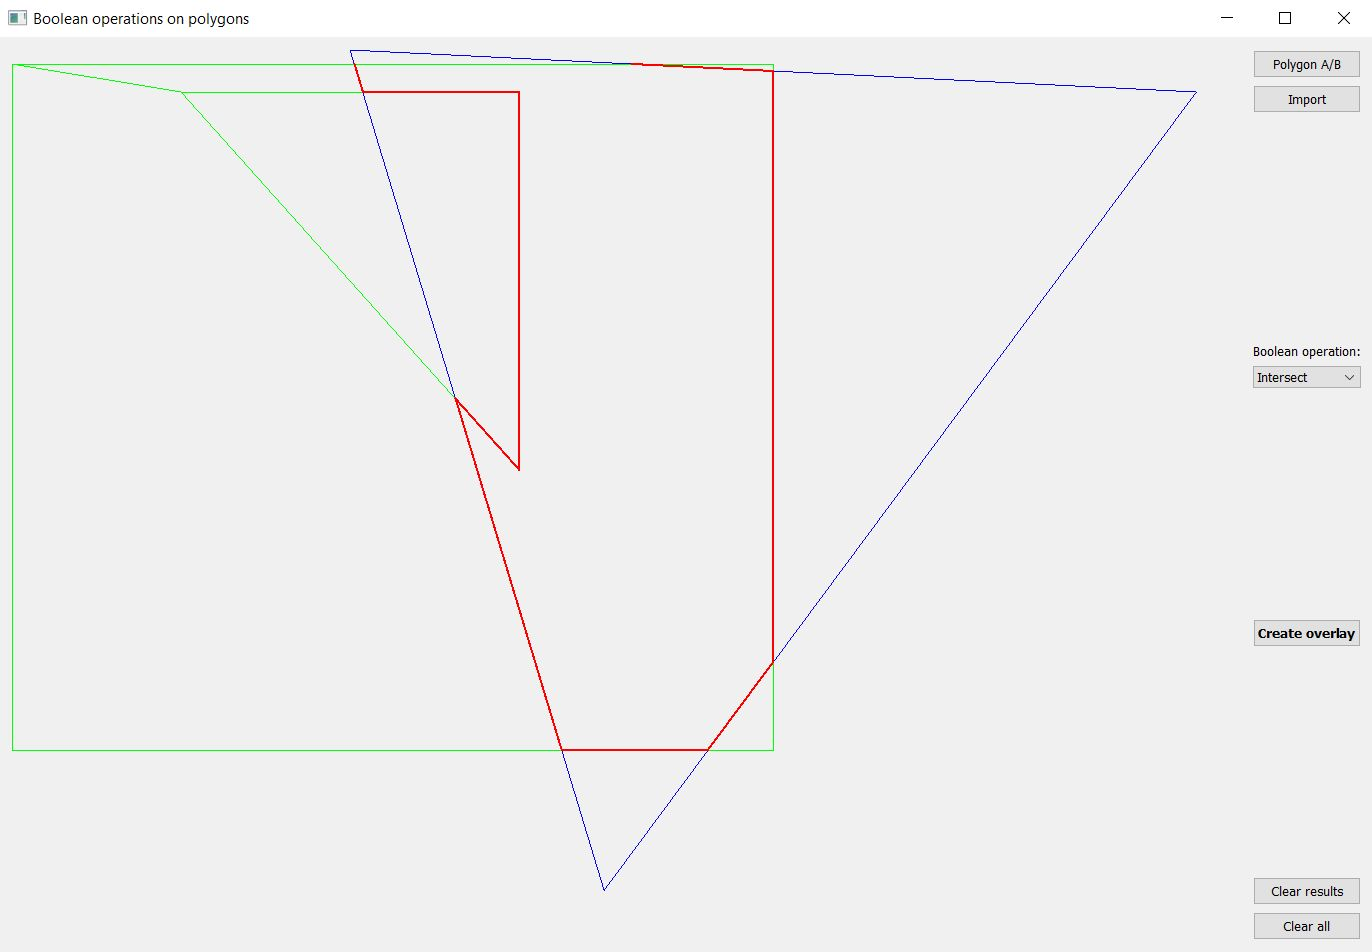
\includegraphics[width=10cm]{t5.jpg}
	\caption{Chybný výsledek pro průnik polygonů.}
\end{figure}

\section{Závěr}
Aplikace provádí nad zadanou množinou vrcholů dvou polygonů množinové operace. Pro "běžné" polygony je výsledný výstup aplikace správný a korektní. Problematické situace popsané v kapitole \textit{5} jsou ošetřeny.  

\section{Náměty pro vylepšení} 
Vylepšení aplikace by bylo možné vytvořením funkcí množinových operací pro více polygonů najednou.\\
\\
Vhodné by bylo také odladění situace kdy polygon obsahuje prázdný polygon ("díru"). Tento problematický případ není v úloze vyřešen.\\
\\
Pro pokrytí většího pole užívání aplikace by také bylo vhodné přidat další funkce jako například konstrukce offsetu.\\
\\
Jednoduchým vylepšením by bylo také přidání množinových operací pro úsečky importované z textového souboru. V aktuální verzi aplikace se takovýto vstup nenačte. Úsečky zadané grafikou cestou zobrazeny jsou, ovšem v případě například průniku je výsledek prázdný vektor hran. 

\section{Reference}

\begin{enumerate}

\item  BAYER, Tomáš. Metody konstrukce konvexní obálky [online][cit. 5.11.2019]. \\
Dostupné z: https://web.natur.cuni.cz/~bayertom/images/courses/Adk/adk4.pdf \\

\item  Matematika.cz [online][cit. 11.12.2019]. \\
Dostupné z: matematika.cz\\

\item  MatFyz.jeCool.net [online][cit. 11.12.2019]. \\
Dostupné z: www.matfyz.jecool.net\\


\end{enumerate}
\end{document}



 